\documentclass[12pt, letterpaper]{article}
\usepackage[titletoc,title]{appendix}
\usepackage{color}
\usepackage{booktabs}
\usepackage[usenames,dvipsnames,svgnames,table]{xcolor}
\definecolor{dark-red}{rgb}{0.75,0.10,0.10}
\usepackage[margin=1in]{geometry}
\usepackage[linkcolor=dark-red,
            colorlinks=true,
            urlcolor=blue,
            pdfstartview={XYZ null null 1.00},
            pdfpagemode=UseNone,
            citecolor={dark-red},
            pdftitle={Ideological Representation}]{hyperref}
%\usepackage{biblatex}
\usepackage{multibib}
\usepackage{longtable}
\usepackage{lmodern}
\usepackage[utf8x]{inputenc}
\usepackage{dcolumn}
\usepackage{geometry} % see geometry.pdf on how to lay out the page. There's lots.
\geometry{letterpaper}               % This is 8.5x11 paper. Options are a4paper or a5paper or other...
\usepackage{graphicx}                % Handles inclusion of major graphics formats and allows use of
\usepackage{amsfonts,amssymb,amsbsy}
\usepackage{amsxtra}
\usepackage{natbib}
\usepackage{verbatim}
\setcitestyle{round,semicolon,aysep={},yysep={;}}
\usepackage{setspace}        % Permits line spacing control. Options are \doublespacing, \onehalfspace
\usepackage{sectsty}         % Permits control of section header styles
\usepackage{lscape}
\usepackage{fancyhdr}        % Permits header customization. See header section below.
\usepackage{url}             % Correctly formats URLs with the \url{} tag
\usepackage{fullpage}        %1-inch margins
\usepackage{multirow}
\usepackage{rotating}
\setlength{\parindent}{3em}

%\usepackage[T1]{fontenc}
%\usepackage{bm}
%\usepackage{libertine}
\usepackage{chngcntr}

% Caption
\usepackage[hang, font=small,skip=0pt, labelfont={bf}]{caption}
\usepackage{subcaption}

% tt font issues
% \renewcommand*{\ttdefault}{qcr}
\renewcommand{\ttdefault}{pcr}

\usepackage{lscape}
\renewcommand{\textfraction}{0}
\renewcommand{\topfraction}{0.95}
\renewcommand{\bottomfraction}{0.95}
\renewcommand{\floatpagefraction}{0.40}
\setcounter{totalnumber}{5}
\makeatletter
\providecommand\phantomcaption{\caption@refstepcounter\@captype}
\makeatother

\title{Extreme Recall: Which Politicians Come to Mind?\\\vspace{10mm}}
\date{September 10, 2026}

\author{Gaurav Sood\thanks{Gaurav can be reached at: \href{mailto:gsood07@gmail.com}{\texttt{gsood07@gmail.com}}.}}

\begin{document}
\newcommand{\sampleAgeYoung}{23.1}
\newcommand{\sampleAgeMiddle}{41.9}
\newcommand{\sampleAgeOlder}{35.0}
\newcommand{\sampleAdvanced}{10.8}
\newcommand{\sampleBachelor}{41.7}
\newcommand{\sampleHighSchool}{11.1}
\newcommand{\sampleCollege}{36.3}
\newcommand{\sampleFemale}{46.8}
\newcommand{\sampleMale}{53.2}
\newcommand{\sampleHispanic}{5.0}
\newcommand{\sampleBlack}{4.7}
\newcommand{\sampleOtherRace}{2.2}
\newcommand{\sampleNative}{1.0}
\newcommand{\sampleWhite}{87.9}
\newcommand{\sampleDemocrat}{56.8}
\newcommand{\sampleIndependent}{12.1}
\newcommand{\sampleRepublican}{31.0}
\newcommand{\sampleAsianPacific}{4.3}
\newcommand{\sampleLessHighSchool}{0.0}
\newcommand{\scoreMentions}{1737}
\newcommand{\scoreRespondents}{344}
\newcommand{\ratedMentions}{1202}
\newcommand{\ratedRespondents}{339}
\newcommand{\partisanMentions}{1526}
\newcommand{\partisanRespondents}{299}
\newcommand{\stageMentions}{1603}
\newcommand{\stageRespondents}{298}
\newcommand{\freeGapChange}{0.000}
\newcommand{\freeGapLower}{-0.033}
\newcommand{\freeGapUpper}{0.033}
\newcommand{\freeGapP}{0.998}
\newcommand{\promptedGapChange}{-0.043}
\newcommand{\promptedGapLower}{-0.077}
\newcommand{\promptedGapUpper}{-0.009}
\newcommand{\promptedGapP}{0.012}

\maketitle

\begin{comment}

setwd(paste0(githubdir, "extreme_recall/ms"))
tools::texi2dvi("extreme_recall.tex", pdf = TRUE, clean = TRUE)
setwd(basedir)

\end{comment}
\doublespacing

In November 2013, we surveyed participants through Amazon's Mechanical Turk \citep[see][]{berinsky2012}; \scoreRespondents{} respondents contribute identified, score-matched free recalls to the analysis. (See \ref{si_survey_dem} for a description of how we processed this data, and comparison to population benchmarks.) We asked the respondents, ``When you think about the Democratic (Republican) party, which political leader(s) first come to mind? Name up to three.'' We followed the open-ended question with a multiple-choice question that presented respondents a list of names and photos of political leaders and asked the respondents ``Is there another political leader that you haven't mentioned already who immediately comes to mind when you think about the Democratic (Republican) party?'' Among the Democrats, people choose between, Joseph Biden, Barney Frank, Bill Clinton, Hillary Clinton, Harry Reid, Ted Kennedy, Franklin Roosevelt, John Kerry, John Kennedy, Nancy Pelosi, Al Gore, Barack Obama. And among Republicans, between, Paul Ryan, John McCain, Rand Paul, Sarah Palin, Ronald Reagan, George W. Bush, John Boehner, Jeb Bush, Michele Bachmann, Ted Cruz, Chris Christie, Marco Rubio, Eric Cantor, Mitt Romney, and Mitch McConnell. We paired the responses with CF-Scores \citep{bonica2013}.

Respondents rated the first two freely recalled names and the prompted selection from each party on a seven-point liberal--conservative scale. There was no rating of the third free recall. Our primary rating analysis uses free recalls; the appendix also reports prompted selections and the pooled sample.

We find that people are likelier to recall prominent politicians (see Figure \ref{fig:fig1}). People recall politicians with more extreme CF-scores earlier and tend to rate recalled politicians toward their party's ideological endpoint (see \ref{si_recall}). These comparisons describe recall order and perceived ideological position; they do not establish whether recalled politicians are more extreme than Congress or whether respondents misperceive their positions.

\begin{figure}[ht]
  \centering
  \caption{Distribution of Recall of Politicians. The horizontal axis counts identified, score-matched free recalls across all three positions.}
  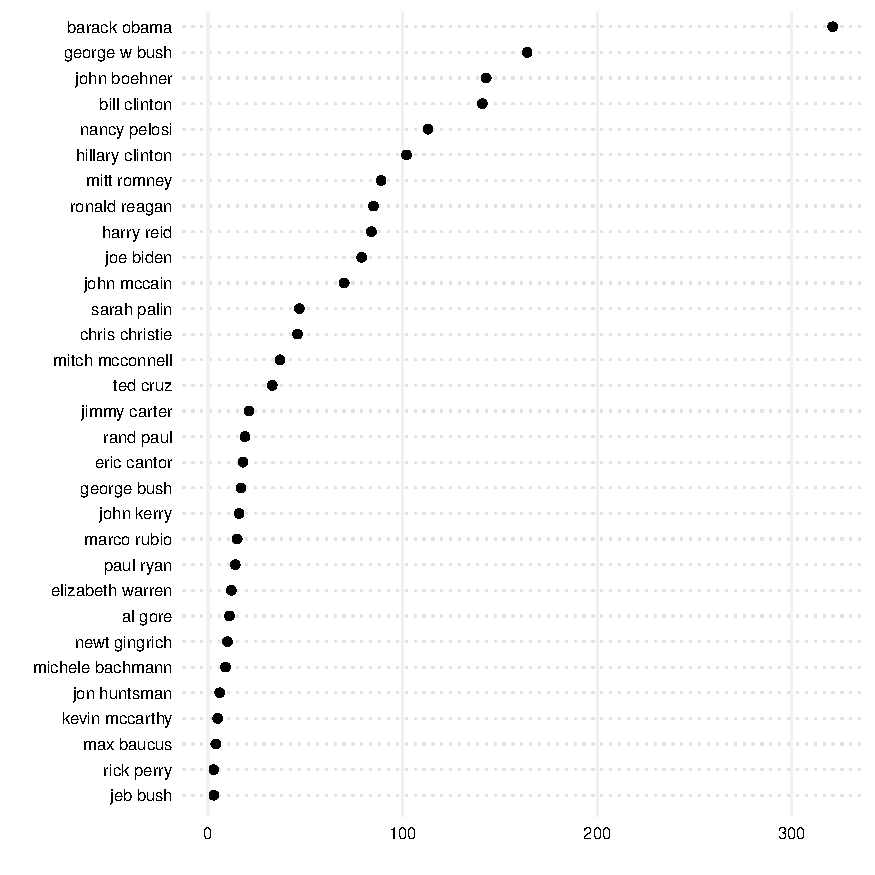
\includegraphics[width=.75\textwidth]{../figs/survey/names_tally.pdf}
  \label{fig:fig1}
\end{figure}

\clearpage

\bibliographystyle{apsr}
\bibliography{polarnews}
\clearpage

\clearpage
\appendix
\renewcommand{\thesection}{SI \arabic{section}}
\setcounter{table}{0}\renewcommand\thetable{\thesection.\arabic{table}}
\setcounter{figure}{0}\renewcommand\thefigure{\thesection.\arabic{figure}}
\counterwithin{figure}{section}

\begin{center}
\Large{Supporting Information}
\end{center}

\section{Survey data}

Because the answers to the politician recall survey questions were open-ended (respondents typed in names), the responses were quite ``noisy'' (in addition to misspellings, some respondents just used last names, some just first names, etc) so we had to take several steps to address this. The historical coding began with politicians whose exact name was used at least 3 times for at least one of the recall questions. Then, to determine whether other respondents were attempting to refer to these politicians, we checked whether the respondent referred to the same last name (for unique last names), common misspellings of the last or first names (oboma, reed, hilary), and common stems for very difficult to spell names (boe or boh for boehner, mccon for mcconnell). The revised analysis applies the union of these historical name assignments consistently across free-recall positions. We retain the historical defaults for ambiguous Bush and Clinton responses: senior or H.W. cues identify George H.W. Bush, other ambiguous Bush responses identify George W. Bush, and 'clinton' identifies Bill Clinton. Explicit 'Jeb Bush' responses identify Jeb Bush. Prompted selections use the identities on the menu. These defaults are coding conventions for ambiguous free responses.

The analysis uses the archived static CF-score for each identified politician. Prompted selections with an available score are retained, including Jeb Bush, Ted Kennedy, and Barney Frank; John F. Kennedy and Franklin D. Roosevelt have no verified score in the archived file. Free-recall name assignments otherwise retain the historical roster. The unit of analysis is a politician--respondent mention. Means weight mentions equally, and uncertainty is clustered by respondent. We use ordinary least squares with a small-sample cluster correction and $t(G-1)$ inference, where $G$ is the number of respondents in the model. Independents contribute to descriptive means but are excluded from in-party/out-party comparisons. Recall position and elicitation stage enter as categories; reported contrasts are unadjusted for multiple comparisons.

Table ~\ref{si_survey_dem} provides a synopsis.

\begin{table}[ht]
\small
\caption{Sample Demographics Compared to Benchmarks}
\centering
\label{si_survey_dem}
\begin{tabular}{l c c c}
\hline
& Sample & 2012 ANES & 2010 Census\\
\hline
& & &\\
\textbf{Age} & & &\\
% External ANES/Census benchmark values are retained from the historical draft.
18-29 & \sampleAgeYoung\% & & 19.2\%\\
30-49 & \sampleAgeMiddle\% & & 31.7\%\\
50+ & \sampleAgeOlder\% & & 49.2\%\\
& & &\\
\textbf{Gender} & & &\\
Male & \sampleMale\% & & 49.1\%\\
Female & \sampleFemale\% & & 50.9\%\\
& & &\\
\textbf{Race/Ethnicity} & & &\\
White/Caucasian & \sampleWhite\% & & 63.7\% \\
Black/African-American & \sampleBlack\% & & 12.2\%\\
Asian/PI & \sampleAsianPacific\% & & 4.8\%\\
Hispanic/Latino & \sampleHispanic\% & & 16.4\%\\
Native American & \sampleNative\% & & 1.1\%\\
Other/more than one & \sampleOtherRace\% & & 6.2\%\\
& & &\\
\textbf{Education} & & &\\
Less than HS degree & \sampleLessHighSchool\% & & 8.9\%\\
High school/GED & \sampleHighSchool\% & & 31.0\%\\
Some college/2-year degree & \sampleCollege\% & &28.0\%\\
4-year college degree & \sampleBachelor\% & & 18.0\%\\
Graduate/professional degree & \sampleAdvanced\% & & 9.3\%\\
& & &\\
\textbf{Party Identification} & & &\\
Democratic (inc. leaners) & \sampleDemocrat\% & 49.0\% &\\
Republican (inc. leaners) & \sampleRepublican\% & 39.0\% &\\
No party preference/Other & \sampleIndependent\% & 11.9\% &\\
\hline
\end{tabular}
\caption*{Note: Sample statistics are for the free-recall analysis, with N=\scoreMentions{} mentions from \scoreRespondents{} respondents. Respondents who recalled more identified politicians receive more weight. White/Caucasian includes Hispanic respondents in the survey but is non-Hispanic for the Census benchmark. Hispanic origin is recorded separately from race in the survey.}
\end{table}
\clearpage

\subsection{Recall Results}
\label{si_recall}
CF-scores are oriented toward the recalled politician's party: Democratic scores are multiplied by $-1$, and Republican scores retain their sign. First recalls have higher party-directed CF-scores than later recalls (Table~\ref{tab:recall_order}). These comparisons condition on the supplied score estimates.

\begin{table}[ht]
\centering
\small
\caption{CF-score Differences by Free-recall Position}
\label{tab:recall_order}

\begin{tabular}{llrl}
\toprule
Party & Comparison & Difference & 95\% CI\\
\midrule
In party & Second minus first & -0.218 & {}[-0.260, -0.176]\\
In party & Third minus first & -0.194 & {}[-0.237, -0.151]\\
Out party & Second minus first & -0.141 & {}[-0.183, -0.099]\\
Out party & Third minus first & -0.114 & {}[-0.159, -0.069]\\
\bottomrule
\end{tabular}

\caption*{Note: Differences are relative to the first free recall, with respondent-clustered 95\% confidence intervals. The model includes \partisanMentions{} mentions from \partisanRespondents{} Democratic or Republican respondents.}
\end{table}

Ratings are oriented toward the recalled politician's party and rescaled from the seven-point slider: 0 is the opposite party's ideological endpoint, 0.5 is moderate, and 1 is the expected party's endpoint. Table~\ref{tab:ratings} reports means for the primary free-recall sample and the prompted-selection comparison. These ratings describe perceived ideological position; the rating scale and CF-score scale do not supply a calibrated measure of perceptual error.

\begin{table}[ht]
\centering
\small
\caption{Perceived Ideological Position by Elicitation Task}
\label{tab:ratings}

\begin{tabular}{lrrrl}
\toprule
Sample & Ratings & Respondents & Mean & 95\% CI\\
\midrule
Free recall & 1202 & 339 & 0.802 & {}[0.789, 0.815]\\
Prompted & 633 & 343 & 0.769 & {}[0.752, 0.787]\\
Both tasks & 1835 & 343 & 0.791 & {}[0.778, 0.804]\\
\bottomrule
\end{tabular}

\caption*{Note: Mention-weighted means with respondent-clustered 95\% confidence intervals. Free recall includes the first two names from each party. Prompted selections are matched to the actual selected name and its score. Independents are included.}
\end{table}

Table~\ref{tab:party_gaps} compares out-party and in-party ratings at each stage. The gap changes by \freeGapChange{} between the first and second free recall (95\% CI [\freeGapLower, \freeGapUpper]; $p=\freeGapP$). Between the first free recall and the prompted selection, the gap changes by \promptedGapChange{} (95\% CI [\promptedGapLower, \promptedGapUpper]; $p=\promptedGapP$). The latter compares elicitation tasks involving different selected politicians; it is not a third free-recall position or an estimate of the causal effect of prompting.

\begin{table}[ht]
\centering
\small
\caption{Out-party Minus In-party Rating Gaps}
\label{tab:party_gaps}

\begin{tabular}{lrl}
\toprule
Stage & Gap & 95\% CI\\
\midrule
First free recall & 0.107 & {}[0.082, 0.133]\\
Second free recall & 0.107 & {}[0.078, 0.136]\\
Prompted selection & 0.064 & {}[0.031, 0.097]\\
\bottomrule
\end{tabular}

\caption*{Note: Gaps and respondent-clustered 95\% confidence intervals come from the party-by-stage model with \stageMentions{} ratings from \stageRespondents{} Democratic or Republican respondents.}
\end{table}

\end{document}
